Για να αποτυπωθεί η επίδραση της αρχικής θερμοκρασίας των ελαστικών στις επιδόσεις ενός γύρου, εκτελέστηκαν δύο γύροι με ομοιόμορφα αρχικά $T_{\mathrm{init}}=30\,^\circ\mathrm{C}$ (ψυχρός γύρος) και $T_{\mathrm{init}}=90\,^\circ\mathrm{C}$ (θερμός γύρος). Οι χρόνοι γύρου που προέκυψαν είναι $82.842\,\mathrm{s}$ και $79.822\,\mathrm{s}$ αντίστοιχα, δηλαδή διαφορά $-3.020\,\mathrm{s}$ υπέρ του θερμού γύρου. Αυτή η διαφορά κάνει εμφανή τη σημασία της προθέρμανσης των ελαστικών. Τα αποτελέσματα του σχήματος \ref{fig:hotVsCold_tempPerTyre} δείχνουν την προθέρμανση ελαστικών στον ψυχρό γύρο. Στην προσομοίωση του θερμού γύρου, τα ελαστικά βρίσκονται ήδη σε μόνιμη κατάσταση, δηλαδή η θερμοκρασία τους στο τέλος του γύρου έχει σταθεροποιηθεί, ενώ τα ελαστικά του ψυχρού γύρου φτάνουν σε μόνιμη κατάσταση μέσα σε μόλις έναν γύρο. Η γρήγορη χρονική σταθερά των ελαστικών πιθανότατα οφείλεται στη μοντελοποίηση μόνο της θερμικής μάζας του πέλματος. Στην πραγματικότητα, ο σκελετός του ελαστικού έχει πολύ μεγαλύτερη θερμική μάζα και χρειάζεται περισσότερο χρόνο για να φτάσει στη θερμοκρασία λειτουργίας.\\[8pt]

\begin{figure}[htbp!]
    \centering
    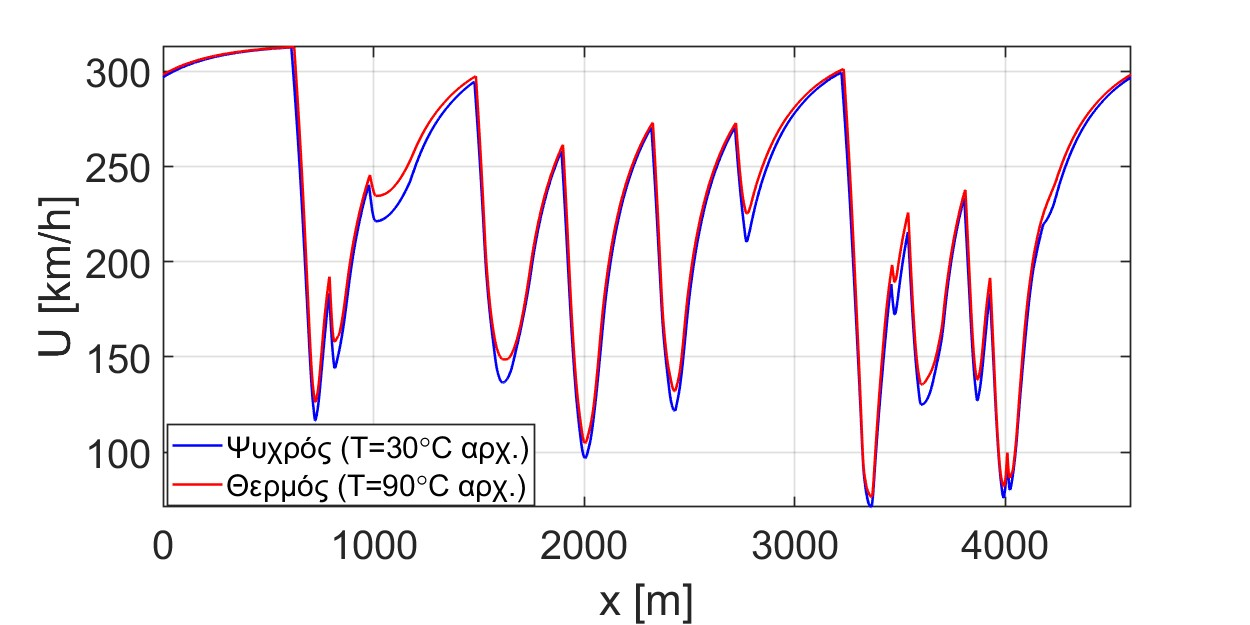
\includegraphics[width=0.85\textwidth]{figures/hotVsCold/vel_coldVsHot.jpg}
    \caption{Προφίλ ταχύτητας $U(x)$ για ψυχρό ($30\,^\circ\mathrm{C}$) και θερμό ($90\,^\circ\mathrm{C}$) γύρο.}
    \label{fig:hotVsCold_vel}
\end{figure}

\begin{figure}[htbp!]
    \centering
    \begin{subfigure}[t]{0.48\textwidth}
        \centering
        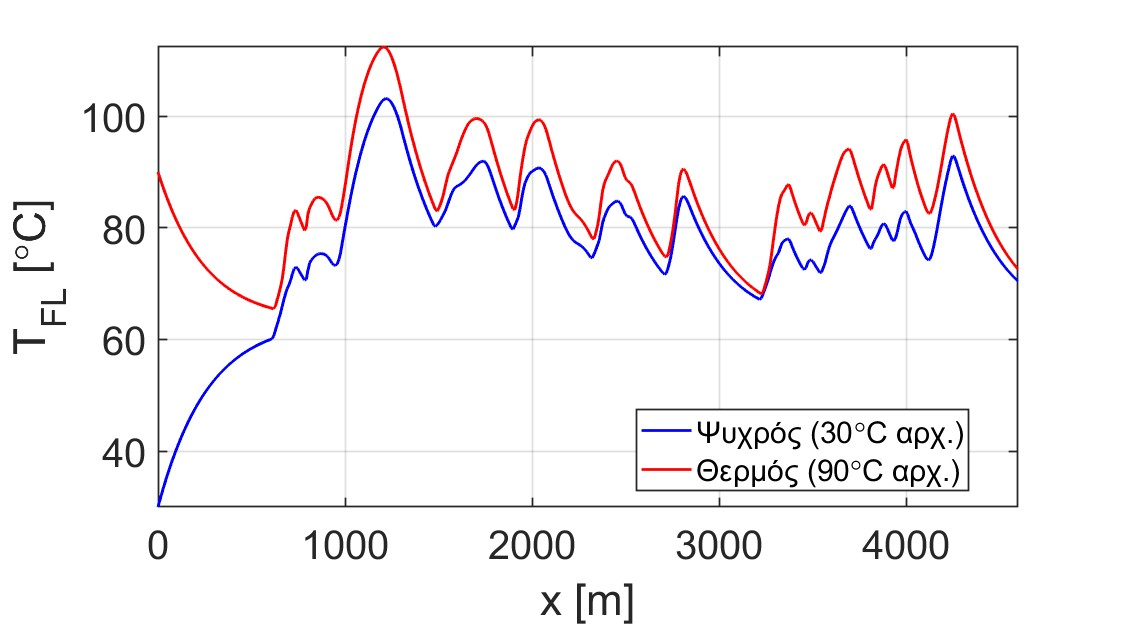
\includegraphics[width=\textwidth]{figures/hotVsCold/T_coldVsHot_FL.jpg}
    \end{subfigure}
    \hfill
    \begin{subfigure}[t]{0.48\textwidth}
        \centering
        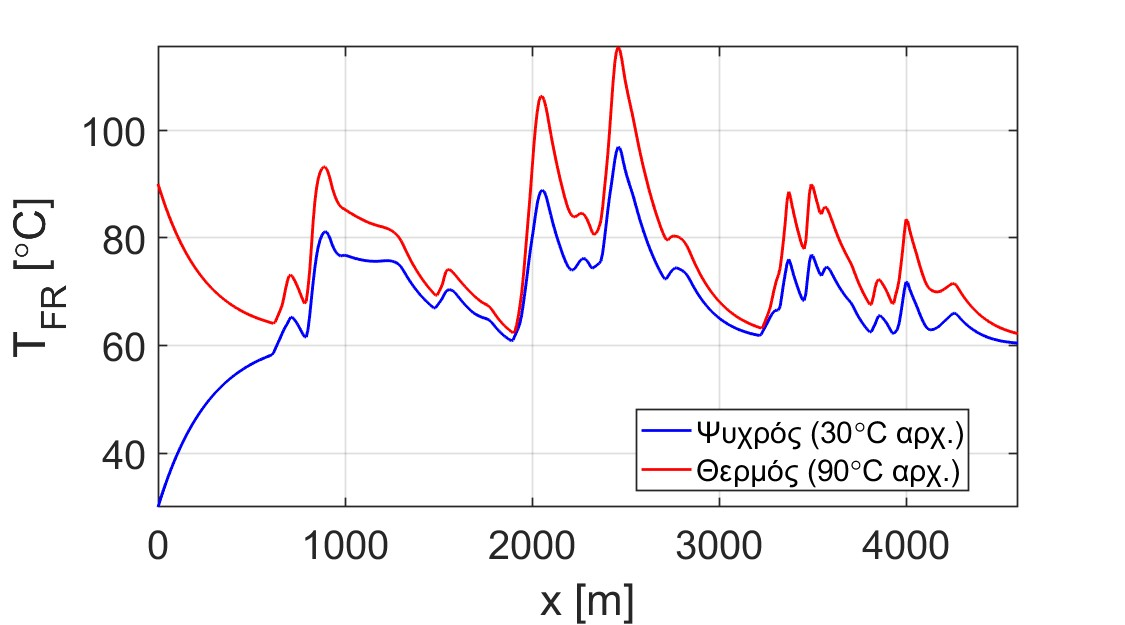
\includegraphics[width=\textwidth]{figures/hotVsCold/T_coldVsHot_FR.jpg}
    \end{subfigure}

    \vspace{0.5em}

    \begin{subfigure}[t]{0.48\textwidth}
        \centering
        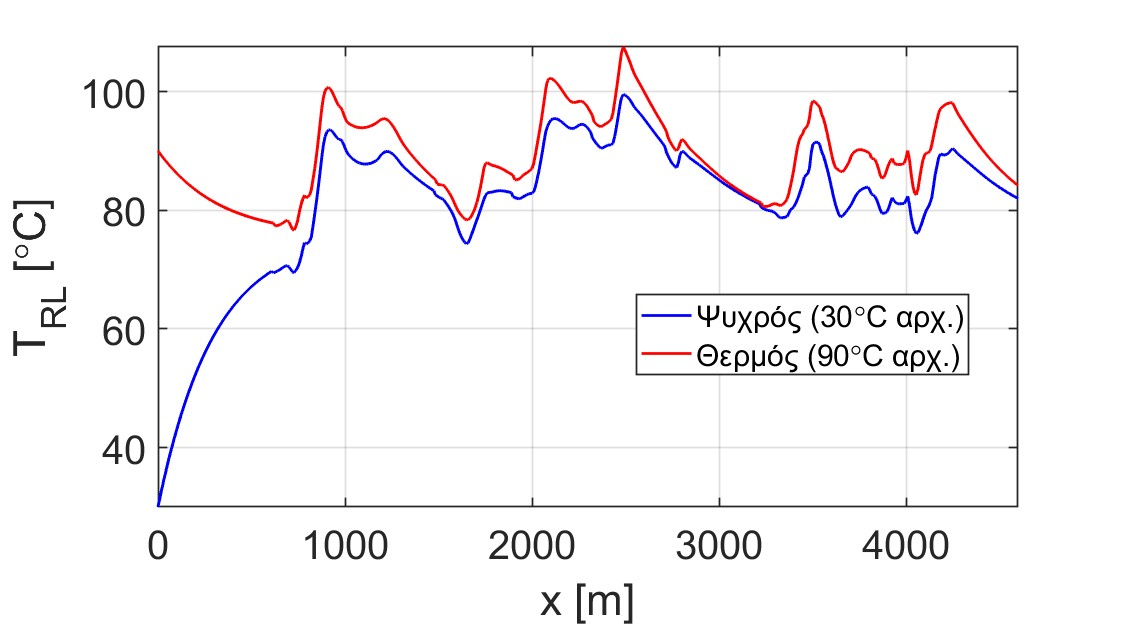
\includegraphics[width=\textwidth]{figures/hotVsCold/T_coldVsHot_RL.jpg}
    \end{subfigure}
    \hfill
    \begin{subfigure}[t]{0.48\textwidth}
        \centering
        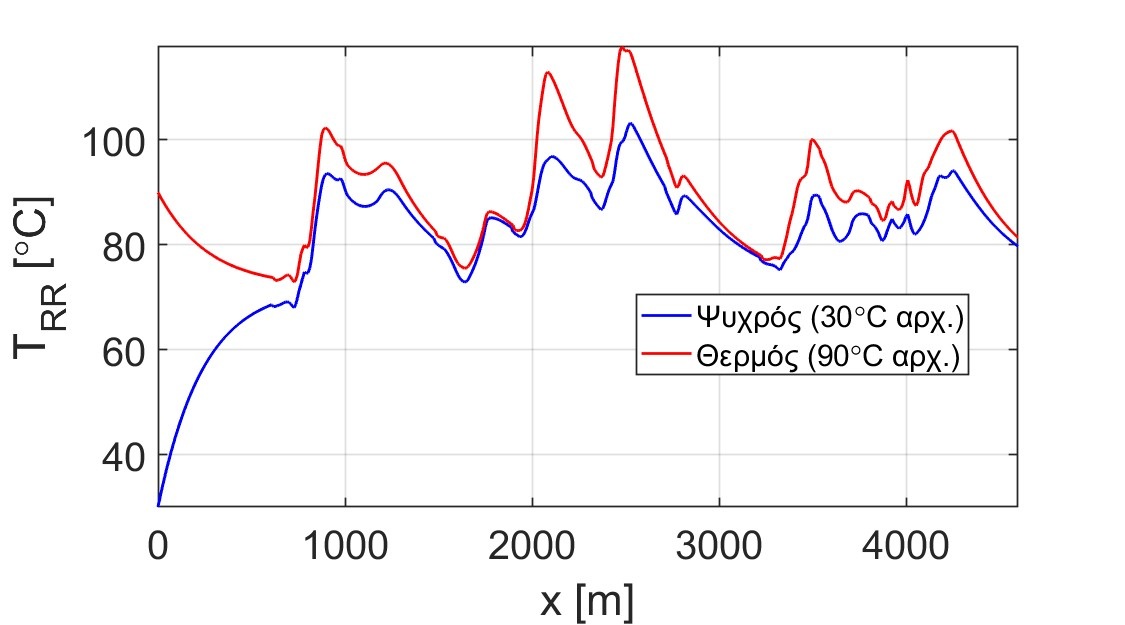
\includegraphics[width=\textwidth]{figures/hotVsCold/T_coldVsHot_RR.jpg}
    \end{subfigure}
    \caption{Εξέλιξη θερμοκρασίας $T_i(x)$ ανά ελαστικό για ψυχρό και θερμό γύρο.}
    \label{fig:hotVsCold_tempPerTyre}
\end{figure}

\FloatBarrier
